\documentclass{beamer}

\mode<presentation>{
  \usetheme{Warsaw}
}


\usepackage[spanish,es-tabla,es-nodecimaldot]{babel}
\usepackage{tikz}
\usepackage{pgf}  %Para realizar figures
\usepackage{xcolor} % Para los colores
\usepackage{enumerate}
\usepackage{graphicx}
\usepackage{array}
\usepackage{cancel}
\usepackage{amssymb}
\usepackage{hyperref}
\usepackage{tcolorbox}  %Cuadros de teoremas


\title[ \hspace{21mm} \insertframenumber \ de \inserttotalframenumber ]
{Distribución binomial}

\subtitle
{Probabilidad, procesos aleatorios e inferencia}

\author[]
{Ana Maritza Bello Yáñez}


\institute[Instituto Polit\'ecnico Nacional]
{
  \inst{1}
  Centro de Investigaci\'on en Computaci\'on
  }

\date[Short Occasion]
{\today}

\keywords{}

\begin{document}

% https://www.youtube.com/watch?v=Nl7BsFe4xmY

\begin{frame}
  \titlepage
\end{frame}

\begin{frame}{Distribución Binomial}
  \begin{block}{Definición}
    La función de probabilidad de una distribución binomial se define como la
    probabilidad de que ocurran exactamente $k$ eventos exitosos de $n$ experimentos
    independientes de probabilidad $p$.

    \begin{equation}
      P(k) = C(n,k) p^k q^{n-k}
    \end{equation}
    
    Esto a también es escrito como:
    \begin{equation}
      b(k; n,p) = C(n,k) p^k q^{n-k}
    \end{equation}
    Donde $0 \leq k \leq n$
  \end{block}
  \begin{block}{}
    Probabilidad de "éxito": $p$

    Probabilidad de "fracaso": $q = 1 - p$
  \end{block}
\end{frame}

\begin{frame}{Eventos tipo Bernoulli}
  \begin{block}{Definición}
    Eventos en los cuales solo existen dos posibles resultados.

    Por ejemplo:

    \begin{itemize}
      \item Tirar una moneda
      \item Lanzar un dardo
      \item Lanzar una tiro para encestar
    \end{itemize}
  \end{block}

  \begin{block}{}
    Probabilidad de "éxito": $p$

    Probabilidad de "fracaso": $q = 1 - p$
  \end{block}

\end{frame}

\begin{frame}{Eventos tipo Bernoulli}

  \begin{block}{Ejemplo}
    Un jugador de baloncesto tiene un 80\% de acierto en tiros libres. Si tira tres
    lanzamientos seguidos, ¿Cuál es la probabilidad de que acierte los tres?
  \end{block}

  \begin{block}{}
    Para un tiro:

    Probabilidad de éxito: $p=0.8$

    Probabilidad de fracaso: $q = 1 - 0.8 = 0.2$
  \end{block}

  \begin{block}{}
    Para tres tiros:

    Probabilidad de éxito: $P(A \cap A \cap A) = p \cdot p \cdot p = 0.8 \cdot 0.8
    \cdot 0.8 = 0.512$

  \end{block}

  \begin{block}{}

    Probabilidad de fracaso: $P(\bar{A} \cap \bar{A} \cap \bar{A}) = q \cdot q \cdot q = 0.2 \cdot 0.2
    \cdot 0.2 = 0.008$

  \end{block}

\end{frame}

\begin{frame}{Distribución Binomial}
  \begin{block}{Ejemplo}
    Un jugador de baloncesto tiene un 80\% de acierto en tiros libres. Si tira tres
    lanzamientos seguidos, ¿Cuál es la probabilidad de que acierte dos de los tres
    lanzamientos?
  \end{block}

  \begin{block}{}
    Sabiendo que:    $p = 0.8$ y  $q = 0.2$

    Entonces:

$P(\text{dos aciertos}) = P(A \cap A \cap \bar{A}) 
                          \cup P(A \cap \bar{A} \cap A)
                          \cup P(\bar{A} \cap A \cap A )$
  \end{block}

  \begin{block}{}  
    Por lo que:
    $P(A \cap A \cap \bar{A}) = p \cdot p \cdot q 
                              = 0.8 \cdot 0.8 \cdot 0.2 
                              = 0.128$
  \end{block}

  \begin{block}{}
    Así:
    
    $P(\text{dos aciertos}) = 0.128 + 0.128 + 0.128 = 3 \cdot 0.128$
  \end{block}
\end{frame}

\begin{frame}{Distribución binomial}
  \begin{block}{Ejemplo}
    Notemos que:

    $P(\text{dos aciertos}) = P(A \cap A \cap \bar{A}) 
                          \cup P(A \cap \bar{A} \cap A)
                          \cup P(\bar{A} \cap A \cap A )$
                          
    Estamos haciendo una combinatoria:

    $C(3,2)$

  \end{block}

  \begin{block}{}
    De esta manera podemos hacerlo para experimentos más grandes. Digamos, ¿cuál
    sería la probabilidad de acertar 3 canastas si hiciera 15 lanzamientos?

    $C(15,3) = 455$
  \end{block}
\end{frame}

\begin{frame}{Distribución binomial}
  \begin{block}{Aplicando la función de probabilidad...}
      Un jugador de baloncesto tiene un 80\% de acierto en tiros libres. Si tira 20
      lanzamientos seguidos, ¿cuál es la probabilidad de que acierte 13 de los
      lanzamientos?
      
    $P(13) = C(20,13) 0.8^{13} \cdot 0.2^{7} = 0.0545$
  \end{block}
\end{frame}

\begin{frame}{Distribución binomial}
  \begin{block}{}
Ahora podemos obtener la distribución de la probabilidad pasando por todos los
valores posibles desde 0 hasta $k$ en:

    $P(k) = C(n,k) p^k q^{n-k}$
  \end{block}

  \begin{center}
  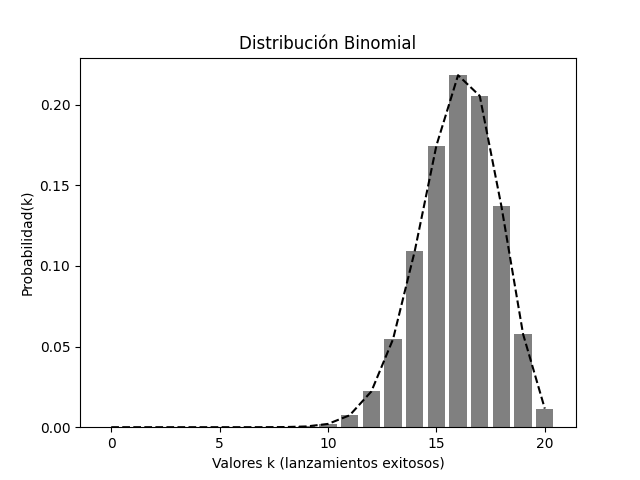
\includegraphics[scale=0.5]{figures/binomial_distribution.png}
  \end{center}
\end{frame}

\begin{frame}
  \begin{block}{Nota}
Cuando el éxito y el fracaso son igualmente probables, la distribución binomial
es una distribución normal. Por lo que si cambiamos el valor de $p$ a 0.5,
obtenemos la siguiente gráfica de distribución normal.
  \end{block}

  \begin{center}
    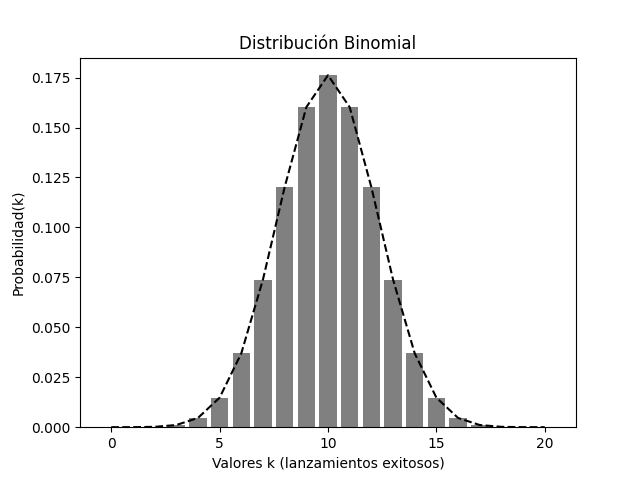
\includegraphics[scale=0.5]{figures/binomial_distribution_normal.png}
  \end{center}

\end{frame}

%\begin{frame}{Definición de distribución}
%    \begin{block}{Definición}
%      Una distribución estadística, o distribución de probabilidad, describe cómo se
%      distribuyen los valores para un campo. En otras palabras, la distribución
%      estadística muestra qué valores son comunes y poco comunes.
%    \end{block}  
%    
%\end{frame}


\end{document}

